
\documentclass{article}

% Copyright (c) 2012 Cies Breijs
%
% The MIT License
%
% Permission is hereby granted, free of charge, to any person obtaining a copy
% of this software and associated documentation files (the "Software"), to deal
% in the Software without restriction, including without limitation the rights
% to use, copy, modify, merge, publish, distribute, sublicense, and/or sell
% copies of the Software, and to permit persons to whom the Software is
% furnished to do so, subject to the following conditions:
%
% The above copyright notice and this permission notice shall be included in
% all copies or substantial portions of the Software.
%
% THE SOFTWARE IS PROVIDED "AS IS", WITHOUT WARRANTY OF ANY KIND, EXPRESS OR
% IMPLIED, INCLUDING BUT NOT LIMITED TO THE WARRANTIES OF MERCHANTABILITY,
% FITNESS FOR A PARTICULAR PURPOSE AND NONINFRINGEMENT. IN NO EVENT SHALL THE
% AUTHORS OR COPYRIGHT HOLDERS BE LIABLE FOR ANY CLAIM, DAMAGES OR OTHER
% LIABILITY, WHETHER IN AN ACTION OF CONTRACT, TORT OR OTHERWISE, ARISING FROM,
% OUT OF OR IN CONNECTION WITH THE SOFTWARE OR THE USE OR OTHER DEALINGS IN THE
% SOFTWARE.

%%% LOAD AND SETUP PACKAGES

\usepackage[margin=0.5in]{geometry} % Adjusts the margins

\usepackage{multicol} % Required for multiple columns of text

\usepackage{mdwlist} % Required to fine tune lists with a inline headings and indented content

\usepackage{relsize} % Required for the \textscale command for custom small caps text

\usepackage[pdftex]{hyperref} % Required for customizing links
\usepackage[dvipsnames]{xcolor} % Required for specifying custom colors
\definecolor{dark-blue}{rgb}{0.15,0.15,0.4} % Defines the dark blue color used for links
\hypersetup{colorlinks,linkcolor={dark-blue},citecolor={dark-blue},urlcolor={dark-blue}} % Assigns the dark blue color to all links in the template

\usepackage{tgpagella} % Use the TeX Gyre Pagella font throughout the document
\usepackage[T1]{fontenc}
\usepackage{microtype} % Slightly tweaks character and word spacings for better typography

\pagestyle{empty} % Stop page numbering

%----------------------------------------------------------------------------------------
%	DEFINE STRUCTURAL COMMANDS
%----------------------------------------------------------------------------------------

\newenvironment{indentsection} % Defines the indentsection environment which indents text in sections titles
{\begin{list}{}{\setlength{\leftmargin}{\newparindent}\setlength{\parsep}{0pt}\setlength{\parskip}{0pt}\setlength{\itemsep}{0pt}\setlength{\topsep}{0pt}}}{\end{list}}

\newcommand*\maintitle[2]{\noindent{\LARGE \textbf{#1}}\ \ \ \emph{#2}\vspace{0.3em}} % Main title (name) with date of birth or subtitle

\newcommand*\roottitle[1]{\subsection*{#1}\vspace{-0.3em}\nopagebreak[4]} % Top level sections in the template

\newcommand{\headedsection}[3]{\nopagebreak[4]\begin{indentsection}\item[]\textscale{1.1}{#1}\hfill#2#3\end{indentsection}\nopagebreak[4]} % Section title used for a new employer

\newcommand{\headedsubsection}[3]{\nopagebreak[4]\begin{indentsection}\item[]\textbf{#1}\hfill\emph{#2}#3\end{indentsection}\nopagebreak[4]} % Section title used for a new position

\newcommand{\bodytext}[1]{\nopagebreak[4]\begin{indentsection}\item[]#1\end{indentsection}\pagebreak[2]} % Body text (indented)

\newcommand{\inlineheadsection}[2]{\begin{basedescript}{\setlength{\leftmargin}{\doubleparindent}}\item[\hspace{\newparindent}\textbf{#1}]#2\end{basedescript}\vspace{-1.7em}} % Section title where body text starts immediately after the title

\newcommand*\acr[1]{\textscale{.85}{#1}} % Custom acronyms command

\newcommand*\bull{\ \ \raisebox{-0.365em}[-1em][-1em]{\textscale{4}{$\cdot$}} \ } % Custom bullet point for separating content

\newlength{\newparindent} % It seems not to work when simply using \parindent...
\addtolength{\newparindent}{\parindent}

\newlength{\doubleparindent} % A double \parindent...
\addtolength{\doubleparindent}{\parindent}

\newcommand{\breakvspace}[1]{\pagebreak[2]\vspace{#1}\pagebreak[2]} % A custom vspace command with custom before and after spacing lengths
\newcommand{\nobreakvspace}[1]{\nopagebreak[4]\vspace{#1}\nopagebreak[4]} % A custom vspace command with custom before and after spacing lengths that do not break the page

\newcommand{\spacedhrule}[2]{\breakvspace{#1}\hrule\nobreakvspace{#2}} % Defines a horizontal line with some vertical space before and after it


\newcommand{\grant}[7]{

\headedsubsection{#1}{#2--#3 (#4)} { % title, start date, end date, source
	\inlineheadsection{Investigators:}{#5}
	\vspace{1.2em}
	\inlineheadsection{Award:}{\$#6 (Share: \$#7)}
	\vspace{1.2em}
}
}

\newcommand{\colabgrant}[8]{

\headedsubsection{#1}{#2--#3 (#4)} { % title, start date, end date, source
	\inlineheadsection{Investigators:}{#5}
	\vspace{1.2em}
	\inlineheadsection{Award:}{\$#6 (Share: \$#7)}
	\vspace{1.2em}
	\inlineheadsection{Collaboration:}{#8}
	\vspace{1.2em}
}
}


\usepackage{pdfpages}
\usepackage{booktabs}
\usepackage{mdwlist}
\usepackage{titlesec}
\usepackage{multirow}
\usepackage{multicol}

\usepackage{graphicx}
\usepackage{amssymb}
\usepackage{epstopdf}
\usepackage{mfirstuc}
\usepackage{hyperref}

\newcommand{\abr}[1]{\textsc{#1}}
\newcommand{\student}[1]{\vspace{.5cm}\fbox{\parbox{0.95\linewidth}{{\small #1}}}\vspace{.5cm}}
\newcommand{\newcite}[2]{\capitalisewords{#1} et al.~\cite{#1-#2}}

\newcommand{\image}[2]{  \begin{center}
\includegraphics[width=.5\linewidth]{images/#1}
\end{center}
  }


\title{Teaching Portfolio}
\author{Jordan Boyd-Graber}
\date{ \today}
\begin{document}

\maketitle

\tableofcontents

\section{Teaching Philosophy}

When the pandemic started, I was on sabbatical.  So I didn't need to
dramatically change the way I taught overnight, thank heavens.
%
Moreover, unlike many of my peers, I
already had a large library of recorded lectures because I've been
doing a flipped classroom for a decade (below is my very first lecture
from 2013).
%
Nevertheless, I still had to change the way I taught.
%
Let me tell you how and why it took me so long to realize it.

\image{first_video_lecture}{}

\section{Flipped Classroom}

If you haven't heard the term before, a flipped classroom is where you
record the lectures, students watch them before class, and then you
use the normal class time to answer questions, work through exercises,
or to talk about tricky issues on homeworks.
%
Following the
suggestions of \newcite{Zappe}{09}, I keep my videos short (around 30
minutes total, edited for concision and broken into 5--15 minute
chunks).

For example, when I talk about topic models, I have videos where I:
  \begin{enumerate}
  \item \href{https://youtu.be/qvr5J9m7Gmw}{discuss with an interlocutor why
    topic modeling is important}
  \item \href{https://www.youtube.com/watch?v=fCmIceNqVog}{introduce what
    topic modeling is;}
  \item \href{https://youtu.be/-tKmyHoVZ-g}{walk through Gibbs sampling to fit
  a topic model from text data;}
  \item \href{https://youtu.be/-tKmyHoVZ-g}{discuss variational inference in
    general; and}
  \item \href{https://youtu.be/smfWKhDcaoA}{then walk through the derivation
    of variational inference for topic models.}
  \end{enumerate}
%
The technical quality of the videos have
improved considerably over the years: I've moved from just a screen
capture to a multiple camera setup with green screen.

Then in class, I answer any questions students have and then we go
through an exercise.
%
For instance, we walk through Gibbs sampling
works for a toy example.
%
Students calculate---by hand---the sampling
equation and go through the process to get the answer.

% A lot of teachers do not like the flipped classroom, and I can
% understand why.
%
% First, it's a lot of work, and it requires planning.
% When I co-taught a flipped classroom with an uninitiated professor, he
% ended up cursing my name for convincing him to take part.

\subsection{Building Bonds}

There's research to suggest that the flipped classroom can help
students engage and retain information~\cite{Zuber-16}, but that's not
the real reason that I do it.
%
I do it because it helps me get to know the students better.  Computer
science is the biggest major at Maryland (over three thousand undergrads), and
\abr{ai}-adjacent fields are even more popular within that major, so my
classes are getting pretty darn big.
%
If I didn't do a flipped
classroom, I would know so many fewer students.

And the flipped classroom also helps form bonds between students.
%
When I was an undergrad, I wanted to take organic chemistry even
though I was a history / \abr{cs} major.
%
That failed because studying for
that class was pretty social, and I was not a chemistry major, so I
didn't have an existing support network coming in.
%
Now that I'm a
professor, one of the reasons I like the flipped classroom is that it
forces people to talk to each other to figure out what questions they
want to ask, work together to solve practice problems, etc.
%
Those
groups and those connections often carry over to homework groups and
project groups.

And this helps me serve the few iSchool, Linguistics, and other ``oddball''
students who are exploring something unfamiliar and---like 2003 Jordan trying out
organic chemistry---don't have an established buddy group (which many of the
CS students have).  The flipped classroom helps them get to know the people
who can help them survive and thrive in the course.

When I once I fell off the wagon and went back to a ``normal'' lecture
mode in 2016 because it was my first time teaching a class, it had a
hundred people, and I had no TA.  I was told that students coming in
would know Python.  But it turned out that a big contingent had only
played around with the language for a week or two and were unprepared!
Because I didn't flip the classroom, I only found out when they were turning in the first homework! This wouldn't have happened in a flipped classroom where
I could see that the struggle was real in front of my own eyes.

So back to March 2020. To make sure that I did not miss out on
creating educational content, I started creating a weekly pub quiz to
replace quiz canceled by our usual haunt, closed of course by the
pandemic.  And as the pandemic dragged on and on, I learned how to
create interactive, fun environments that got small groups to discuss
problems, come to a solution, and then share it with the group---the
same thing that I'd need to move the interactive portion of flipped
classes online.  And I
learned how to broadcast with a green screen in real-time and share
multimedia with the group.  (All outlined in \href{https://docs.google.com/document/d/1YesfpZ_-b2mT3BkTrlOLD5epZxz4uF1DqUkHZHrn344/edit?usp=sharing}{this document} that formed
the foundation for pandemic-era pub quizzes.)  I used the same
format and technology for \href{https://sites.google.com/view/qanta/past-events/neurips-2020-efficient-qa}{Google's Efficient QA competition} that I
hosted in December 2020.

\image{efficient_qa}{}

\section{Hybrid Classrooms}

Given all of this, I thought that when we (mostly) returned into hybrid
classrooms (i.e., some students in the classroom some were on Zoom), I'd be
all set for the new world of teaching.  After all, I had already mastered
asynchronous videos, and I had practiced online-only interactions.  I was not
ready, however.  In a real classroom, I could tell when a student was lost or
disengaged.  This is not true when many students are on Zoom.  A hybrid
classroom has a particularly pernicious failure mode: a student doesn't watch
the videos, joins online, gets lost in the discussion, and then silently
disengages.

To make matters worse, many of the improved learning outcomes in
flipped classrooms come from regular quizzes~\cite{tune-13}, which if
nothing else would have diagnosed students disengaging. In an attempt
to make classroom management easier and to lighten the burden on
students, I suspended quizzes.  Another mistake!

And this isn't transitory.  Although it emerged under unpleasant
circumstances, I think the hybrid classroom is going to be with us for
a while for good reasons.  Even after we returned to classrooms,
students were struggling with visa issues, health issues beyond COVID,
were attending conferences, were at home for a wedding, or were snowed
in.  It makes the classroom more equitable and flexible.

And like many faculty, I'm still developing best practice on how to do
this.  I encourage people to keep their cameras on and I make a big
deal of the 10\% participation grade.  This creates some
annoyances\dots for example, students asking questions for the sake of
hitting the participation quota rather than actually wanting
information, but it's a small price to pay.  I'm proud that after a
shaky start and uncooperative \abr{av}, I'm getting good engagement
from both in-person and Zoom students.

\section{Assignments}

But teaching is not just about lectures.  My courses typically have a
few small, practical assignments (typically three to five), a midterm,
and a course project.

The assignments give continuity to the class and allow students to
practice skills introduced in the class; I encourage students to work
together to solve homework problems.
%
For example, students put together a logistic regression classifier to
determine if an answer to a question is correct or not.  In my mind,
an ideal homework assignment has an easy to achieve initial goal but
leaves room for exploration.  Returning to the logistic regression
example, just implementing stochastic gradient descent challenges some
students (and they stop there), but for students who want to explore
further, they can try out different step sizes and updating schedules
for extra credit.

The midterm serves as a reality check for both my students and me.  I
design exams with five to six free response questions (of which
students must answer a subset) that synthesize disparate concepts from
the course in a problem context (e.g., for a machine learning course,
proving the \abr{vc} complexity of a simple hypothesis class).  Based
on the results of the midterm, I can identify students that might need
extra help or what areas I need to cover in more detail.

\section{Projects}

I want to make sure that my students can actually use their skills
once they're done with the class.  Thus, I typically end courses with
a project.  It reinforces key concepts from the course, connects those
concepts to the rest of their curriculum and research, and often
serves as a launching point to things that are useful in the real
world.  For undergraduate classes, this is more directed: in one class
they build trivia-playing robots to take on former \textit{Jeopardy!} Champions
or Victoria Groce from the American version of \textit{The
  Chase}.\footnote{\href{https://www.youtube.com/watch?v=dyaR7zT_KKg}{https://www.youtube.com/watch?v=dyaR7zT\_KKg}}  For
graduate courses, projects are more open-ended.  Projects in my
courses have become a comedy troupe's website, have unearthed
previously unknown primary sources on local history, helped students
advance in the workplace, and resulted in academic publications.  As a
testament to the effectiveness of these relationships, after one
graduate course I taught (Computational Linguistics II, UMD CMSC 773),
I ended up publishing papers with four of the eight students.

%% The projects help individuals calibrate the course to their own needs
%% and abilities; because the project is directed toward things they care
%% about, the teams working on the projects typically stretch their
%% abilities more than I could through predefined assignments.

\section{Outreach}

And I like to think that my teaching style has helped learners outside
the University of Maryland make progress toward learning about the
interaction between science and society.  The videos on my YouTube
channel have been viewed a million times and my most popular videos
about fifty thousand times.  This has offered me new connections:
e.g., people who come up to me at conferences to say that they learned
variational inference or TV producers wanting to make a Human
vs. Computer game show.

A major part of my research is making machine learning accessible to
high school students.
%
My human-computer question answering exhibition matches have attracted
thousands of interested high school students in \abr{dc}, Chicago,
Dallas, Atlanta, and Seattle.
%
I've also served as a mentor as a part of Maryland's Bitcamp and
Technica hackathon programs on projects of women and underrepresented
minorities to build \abr{qa} systems.

\image{atlanta_hsnct}{}

Thus, I'm glad that I had to up my game because of the pandemic,
starting with an \textit{ad hoc} trivia game in mid March 2020.  I
think it's a good example of how with technology we can better serve
those who want to learn, whether they're our students or not.  And
while some innovations are a matter of necessity rather than of
careful deliberation and insight, we should still embrace them if they
help students learn better.

\section{Mentoring}

\subsection{Mentoring Undergraduates}

Like everything else, the pandemic has changed the way I work with
undergraduate researchers.
%
I began a ``anyone welcome'' summer virtual internship for
undergraduate students to work on small, bite-sized projects that fit
into a larger research program (usually directed by a mid-career grad
student).
%
Our work with undergraduates has been published in top venues like
\abr{naacl} and \abr{chi}, and the undergraduates I've worked with
have gone on to have successful research careers (e.g., Lester Mackey
became faculty at Stanford before moving to Microsoft Research, Eric
Wallace is now a PhD student at Berkeley).
%
My current star undergraduate student, Chenglei Si (class of 2024) already
has six publications in top venues.

\subsection{Mentoring Graduate Students}

I've graduated seventeen PhD students and am the chair or co-chair for
eight current students.  I like to have a group meeting every other
week with students I'm working with (broadly construed), and
one-on-one meetings as needed with students, typically once a week. In
addition, everyone in my group (me included) sends a weekly e-mail to
the group saying: what they worked on that week; what they plan to work
on next week; anything that's holding them up or blocking their
progress. I use an Internet chat program (Slack) to communicate with remote
students and for lower-latency conversations than e-mail.

In their first year, students typically work on a starter project that
builds on a senior student's work; this often becomes a paper with the
new student as a first author.  From there, I work with the student to
craft a trajectory of papers that will form a foundation for the rest
of their graduate studies.
%% While I'm fairly hands-on with conference
%% and journal submissions, I never edit proposals or dissertations; I
%% provide verbal feedback and suggestions but students must find their
%% own voice in the writing process.

After graduation, my students have gone on to good positions in
industry (e.g., Forough Poursabzi and Ahmed Elgohary at Microsoft
Research; Pedro Rodriguez at \abr{fair}) and academia (e.g., Alvin
Grissom II, Assistant Professor at Haverford; He He, Assistant
Professor at NYU; Mohit Iyyer, Assistant Professor at UMass Amherst).


% \section{What Students Say \dots}

% Below are cherry-picked comments from students either sent as an unsolicited
% e-mail (anonymized and presented with permission) or taken from anonymous course
% evaluations.

% \student{ I just started a new job on Monday as a Librarian at [awesome place].
%   I was hired to catalog a special project with the archives and never thought
%   I'd need anything from [introduction to information technology] \dots And then
%   on the first day we started talking about the database of objects.  When we
%   finally got access to the database, I realized it was entirely a SQL database
%   and had to use everything you taught us last semester to help think of how to
%   run the queries and ask the designer what it is capable of.  }


% \student{
% I actually had a job interview for a professional librarian job this week and it
% was about digital libraries.  They asked me questions about what do I know about
% IP validation, HTML, servers, etc.  Thankfully, fresh out of your class, I was
% able to say ``actually, I know a TON about this stuff! There was a question on
% our midterm about IP validations and everything!''

% I wanted to write to let you know that the things I learned in your class this semester are already having a huge impact on my career.
% }

% \student{I showed the \dots app I made for my final project to my boss, and she
%   ran downstairs to [important person]. He came upstairs to see my app and to
%   talk to me about it. Turns out he has a team researching vendors who could
%   provide our library with a mobile presence much like the one I made for my
%   final project in your class. He was excited to see what I'm capable of and
%   will be putting me in touch with the people on the project. This is a big deal
%   for an entry-level librarian like me.}


\clearpage

\section{Placements}

\subsection{PhD Students}

  \begin{enumerate*}
  \item Michelle Yuan (UMD CMSC, 2018--2022): Multilingual Interactive Topic
  Modeling [Amazon]
      \item Chen Zhao (UMD CMSC, 2018--2022): Algorithms with
        Structure for Answering Complex Questions [New York
        University Shanghai, Assistant Professor]
  \item Yoshinari Fujinuma (Colorado CMSC, 2016--2021): Multilingual
    Dense Representations [Amazon]        
      \item Denis Peskov (UMD CMSC, 2017--2021): Human-in-the-loop
        Data Curation [Princeton University, Postdoc]
\item Pedro Rodriguez (UMD CMSC, 2017--2021): Evaluating Machine
  Intelligence with Question Answering [Meta \textsc{fair}]
\item Shi Feng (UMD CMSC, 2017--2021): User Modeling of Knowledge and
  Ability for Question Answering [George Washington University, Assistant Professor\footnote{Starting Fall 2024}]
\item Ahmed Elgohary (UMD CMSC, 2018-2021): Human Feedback for
  Question Answering [Microsoft Research]
\item Shudong Hao\footnote{Later advised by Michael Paul} (CU CSCI, 2015--2017): Interactive Multilingual
  Topic Modeling [Stevens Institute of Technology, Assistant Professor]
  \item Alison Renner-Smith\footnote{Originally advised by Leah Findlater} (UMD CMSC, 2017--2019): Interactive Topic Modeling [Dataminr]
\item Weiwei Yang (UMD CSCI, 2014--2019; co-advised by Philip Resnik): Linked Topic Models [Meta]
\item Forough Poursabzi-Sangdeh (CU CSCI, 2014--2018): Active Labeling with Topic Models [Microsoft]
\item Kim Glasgow\footnote{Later advised by Yla Tausczik} (UMD iSchool 2011--2014): Social Action in Social Media [JHU APL]
\item Thang Nguyen (UMD CMSC, 2012--2018): Anchor-Based
  Topic Inference [CGI Federal]
\item Alvin Grissom II (CU CSCI, 2012--2017):
  Reinforcement Learning for Feature-wise Language Tasks [Haverford College, Assistant Professor]
\item Mohit Iyyer (UMD CMSC, 2012--2017; co-advised by Hal Daum\'e): Deep Learning for Question
  Answering [University of Massachussetts Amherst,
  Associate Professor]
\item He He (UMD CMSC: 2011--2016; co-advised by Hal Daum\'e): Algorithms that Trade-Off Speed and Accuracy [New York University, Assistant Professor]
\item Viet-An Nguyen (UMD CMSC, 2010--2015; co-advised by Philip Resnik): Detecting Influence in Text [Meta]
\item Ke Zhai (UMD CMSC, 2009--2014): Large Scale Bayesian Inference [Microsoft]
\item Yuening Hu (UMD CMSC: 2009--2014): Interactive Topic Modeling [Google]
\end{enumerate*}


\subsection{MS Students}

\begin{enumerate*}
\item Davis Yoshida (CU APMA, 2016--2017): Domain Adaptation for
  Question Answering [First position: PhD student, TTI-Chicago]
\item You Lu (CU CSCI, 2016--2017): Task-based Evaluation of Topic
  Models [First position: PhD student, Virginia Tech]
\item Alison Smith (UMD CMSC, 2011--2013): Evaluating Interfaces for Interactive Topic Modeling [First position: Dataminr]
\item Brianna Satinoff (UMD CMSC, 2009--2011): Incremental Models for Text Classification [First position: Wellpoint]
\end{enumerate*}


\subsection{BS Students}

    \begin{enumerate*}
    \item Feng Guo (UMD, 2022--2023): Playing Centaur Diplomacy [MS Student, UMD]
  \item Chenglei Si (UMD, 2020--2023): Answer Equivalence [PhD Student, Stanford]        
    \item Andrew Mao (UMD, 2020--2022): Interactive Information Retrieval
      for Online Academic Competitions    [Engineer, Meta]
    \item Naveen Raman (UMD, 2020--2022): Active Learning for Coreference [PhD Student, CMU: Winner, Goldwater Scholarship]
    \item Arjun Akkiraju (UMD, 2020--2021): Generating Adversarial QA Examples     [Apple]
  \item Eric Wallace (UMD, 2018--2019): Generating challenging questions for
    question answering [PhD Student, Berkeley]
  \item Sujith Vishwajith (UMD, 2017--2018): Answer equivalence for question answering [AirBnB]
  \item Davis Yoshida (CU, 2015--2017): Active feature solicitation for question answering [PhD Student, TTI]
  \item Henrik Larsen (CU, 2015--2016): Verb prediction [University of Oslo]
  \item Stephanie Hwa (UMD, 2013--2014): Vector word representations for named entities in question answering [Linkedin]
  \item Danny Bouwman (UMD, 2013--2014): Crowdsourced coreference annotation [Web Developer, The Canton Group]
  \item Kenrick Kin, Joshua Lee, Lester Mackey (Princeton, 2005--2006): Assistive vocabulary devices
    for people with aphasia [Kenrick: Pixar; Joshua: Parachute Health; Lester: MSR]
\end{enumerate*}


\clearpage

\section{Sections Taught from the Last Five Years}

\begin{tabular}{ccccccccccccccccccccc}
\toprule \multirow{2}{*}{ Course } & \multirow{2}{*}{\begin{tabular}{c}
2016 \\
F \\
\end{tabular}} & \multicolumn{2}{c}{2017} & \multicolumn{2}{c}{2018} & \multicolumn{3}{c}{2019} & \multicolumn{3}{c}{2020} & \multicolumn{3}{c}{2021} & \multicolumn{3}{c}{2022} & \multicolumn{2}{c}{2023} & \multirow{2}{*}{ Totals } \\
& & S & F & S & F & S & I & F & S & I & F & S & I & F & S & I & F & S & F & \\
\midrule CMSC389A & & & & 28 & & & & & & & & & & & & & & & & 28 \\
INST414 & & & & 36 & & & & & & & & & & & & & & & & 36 \\
$\mathrm{CMSC} 470$ & & & & & & 38 & & & & & & & & 47 & & & & 70 & & 155 \\
CMSC499A & & & & 1 & & 1 & & & & & 3 & 1 & & 3 & & & & & 2 & 11 \\
CMSC723 & & & & & 53 & & & & & & & 66 & & & & & 65 & & & 184 \\
LING723 & & & & & & & & & & & & 1 & & & & & 1 & & & 2 \\
CMSC726 & & & 58 & & & & & & & & & & & & & & & & & 58 \\
INST735 & & & & & 8 & & & & & & & 4 & & & & & 3 & & & 15 \\
CMSC798 & & & & 1 & 2 & & & 1 & & & & & & 3 & 2 & & 3 & 1 & 2 & 15 \\
INST808 & & & & & & & & & & & 8 & & & & & & & & & 8 \\
CMSC848Q & & & & & & & & & & & & & & & 47 & & & & 21 & 68 \\
CMSC898 & & & 3 & 5 & 7 & 9 & 1 & 5 & 4 & 1 & 5 & 1 & & 2 & 1 & 1 & 2 & 2 & 4 & 53 \\
CMSC899 & 1 & 1 & & & 1 & 1 & & 2 & 3 & 2 & 3 & 7 & 5 & 4 & 2 & 1 & & & & $\mathbf{33}$ \\
  \midrule
Totals  & 1 & 1 & 61 & 71 & 71 & 49 & 1 & 8 & 7 & 3 & 19 & 80 & 5 & 59 & 52 & 2 & 74 & 73 & 29 & 666 \\
\bottomrule
\end{tabular}

\subsection{CMSC 398A: Practical Deep Learning}

\paragraph{Description}
``Deep Learning'' systems, typified by deep neural networks, are increasingly taking over all AI tasks, ranging from language understanding, and speech and image recognition, to machine translation, planning, and even game playing and autonomous driving. As a result, expertise in deep learning is quickly transitioning into a prerequisite in many advanced academic/research settings, and a large advantage in the industrial job market.

This course provides a comprehensive, practical introduction to modern deep learning networks and their applications to AI tasks. Specifically, the course will cover basic concepts in optimization, neural networks,.

\paragraph{Learning Outcomes} By the end of the course, it is expected that students will be able to describe and implement convolutional neural networks (CNN), and recurrent neural networks (RNN), understand the basic concepts of gradient-based optimization, and be able to design and develop deep learning models for tasks that they care about.

Full schedule and topics: \href{https://umd-cs-stics.gitbooks.io/cmsc389a-practical-deep-learning/content/}{Full Schedule and Topics}

\subsection{INST 414: Advanced Data Science}

\begin{itemize*}
\item Sample Lecture: \href{https://www.youtube.com/watch?v=O28U08_yaGU}{Expectations and Entropy}
\item \url{http://users.umiacs.umd.edu/~jbg/teaching/INST_414/}{Full Schedule and Topics}
\end{itemize*}

\paragraph{Description}
This course explores the application of data science techniques to unstructured, real-world datasets including social media and open data sources. The course will focus on techniques and approaches that allow the extraction of information relevant for experts and non-experts in a wide range of areas including smart cities, transportation or public safety.

This course will explore approaches to extract insights from large-scale datasets. The course will cover the complete analytical funnel from data extraction and cleaning to data analysis and insights interpretation and visualization. The data analysis component will focus on techniques in both supervised and unsupervised learning to extract information from datasets. Topics will include clustering, classification, and regression techniques.  Through homework assignments, a project, exams and in-class activities, students will practice working with these techniques and tools to extract relevant information from structured and unstructured data.


\paragraph{Learning Objectives}

\begin{itemize*}
\item Collect and clean large-scale datasets
\item Recognize when a function is a valid probability distribution
\item Manipulate conditional and marginal probability distributions
\item Apply Bayes rule to invert conditional probabilities
\item Describe distributions using standard parameterizations of
\item Use a random number generator to sample from the distribution
\item Given data and an objective function, derive the form of the maximum likelihood parameters for logistic and linear regression
\item Given a parameterization of logistic regression classifiers, output a classification on an example
\item Given training examples, use stochastic gradient to update classifier parameters
\item Correct problems of data representation to improve classification or regression
\item Design training / test data splits that allow effective evaluation of data science algorithms
\item Recognize when a problem can benefit from classification
\item Given a dataset, run k-means clustering or Gaussian mixture models
\item Critically evaluate the accuracy of different algorithms and the appropriateness of a given approach
  \end{itemize*}

  \subsection{CMSC 470: Natural Language Processing}

  \begin{itemize*}
  \item Sample Lecture: \href{https://www.youtube.com/watch?v=A5ounv0D_cs}{tf-idf}
    \item \href{https://users.umiacs.umd.edu/~jbg/teaching/CMSC_470/}{Full Schedule and Topics}
    \end{itemize*}
  
  \paragraph{Description}
Introduction to fundamental techniques for automatically processing and generating natural language with computers. Machine learning techniques, models, and algorithms that enable computers to deal with the ambiguity and implicit structure of natural language. Application of these techniques in a series of assignments designed to address a core application such as question answering or machine translation.

  \paragraph{Learning Objectives}
  Students will understand the modern NLP neural pipeline, starting from stochastic gradient descent on classifiers with sparse representations to transformer models.  Students will implement representations of text using tf-idf, word vectors, and transformers and apply those representations to language modeling for next word prediction and providing useful answers to user input.

  

  

\subsection{LING/CMSC 723/INST 735: Graduate Natural Language Processing (formerly Computational Linguistics)}

\begin{itemize*}
\item Sample Lecture: \href{https://www.youtube.com/watch?v=u7l5hhmdc0M}{Gibbs Sampling Inference for Topic Models}
  \item \href{http://users.umiacs.umd.edu/~jbg/teaching/CMSC_723/}{Full Schedule and Topics}
\end{itemize*}

\paragraph{Description}
Computational linguistics has two main areas: how to build technology that does useful things with human language (this area is usually referred to as "natural language processing", NLP, or sometimes "human language technology"), and how to improve our scientific understanding of how language works using computational methods and models. We will be looking at both, with an emphasis on conceptual understanding, looking at data, and understanding the ways in which the computational study of language differs from other areas in which computational approaches are being used.

\paragraph{Learning Objectives}
By the end of the course, students should understand and implement the typical annotations of the natural language processing pipeline: segmenting characters into words or word pieces, inferring the latent structure of sentences via finite state automata or context free grammars, and classifying text according to a label set.  Moreover, students should have the foundation to implement new algorithms and approaches for natural language processing tasks.


\subsection{CMSC 726: Machine Learning}

\begin{itemize*}
  \item Sample Lecture: \href{https://www.youtube.com/watch?v=Ju2z_WjrIOY}{Structured Predictions}
  \item \href{http://users.umiacs.umd.edu/~jbg/teaching/CMSC_726/}{Full Schedule and Topics}
\end{itemize*}

\paragraph{Description}
This course covers classification algorithms, regression algorithms, unsupervised classification algorithms, and multi-layer representation learning, using theoretical frameworks for proving learning bounds using VC dimension and Rademacher complexity.  Inference and solutions will focus on scalable, online frameworks such as stochastic gradient descent.

\paragraph{Learning Objectives} By the end of this course, you’ll be able to take a problem and analyze it to determine which machine learning techniques are appropriate for solving the problem, how to prepare data to use that solution, apply the solution, and to evaluate the results.  For the most common machine learning techniques, you’ll also be able to implement solutions in Python.



\subsection{INST 808: Quantitative Methods}

\begin{itemize*}
\item Sample Lecture: \href{https://www.youtube.com/watch?v=-lgKvN6kGBk}{Recreating a Classic Visualization from Menard}
  \item \href{http://users.umiacs.umd.edu/~jbg/teaching/INST_808/}{Full Schedule and Topics}
  \end{itemize*}


\paragraph{Description}
Understanding information often requires the application of quantitative methods.  After reviewing essential foundational skills for quantitative analysis: hypothesis testing, manipulating data on a computer, and validating experiments computationally.  We focus on computational quantitative methods instantiated through models that allow you to cluster data for understanding large datasets, label data automatically, and answer questions from information.  These models will be implemented via linear and nonlinear models within a common deep learning framework.

\paragraph{Learning Objectives}
The goal of this course is to provide information science researchers with the quantitative tools necessary to conduct research: to know when a statistical test is appropriate for data analysis, run the appropriate test, and interpret the results; to cluster and analyze continuous and discrete datasets; to beautifully plot data; and to use toolkits for classification and regression.

\subsection{CMSC 848Q: }

\paragraph{Course Description}
Computers have made it possible, even easy, to collect vast amounts of text from a wide variety of sources. It is not always clear, however, how to use those data and how to extract useful information from data. This problem is faced in a tremendous range of scholarly, government, business, medical, and scientific applications. The purpose of this course is to teach some of the best and most general approaches to understand how humans and computers can answer questions with this information.


\paragraph{Learning Objectives}
Students will understand the three major paradigms for question answering systems---retrieval-based systems, generation-based systems, and knowledge-based systems---and implement a QA system on text data.  Students will be able to think critically about the goals of QA datasets for either satisfying information needs or probing knowledge.  The final goal of the course is to conduct novel research in the QA domain.

\begin{itemize*}
\item Sample Lecture: \href{https://www.youtube.com/watch?v=WCIFUJ5oeRA}{Why Watson on Jepardy! was Rigged}
  \item \href{http://users.umiacs.umd.edu/~jbg/teaching/CMSC_848/}{Full Schedule and Topics}
  \end{itemize*}

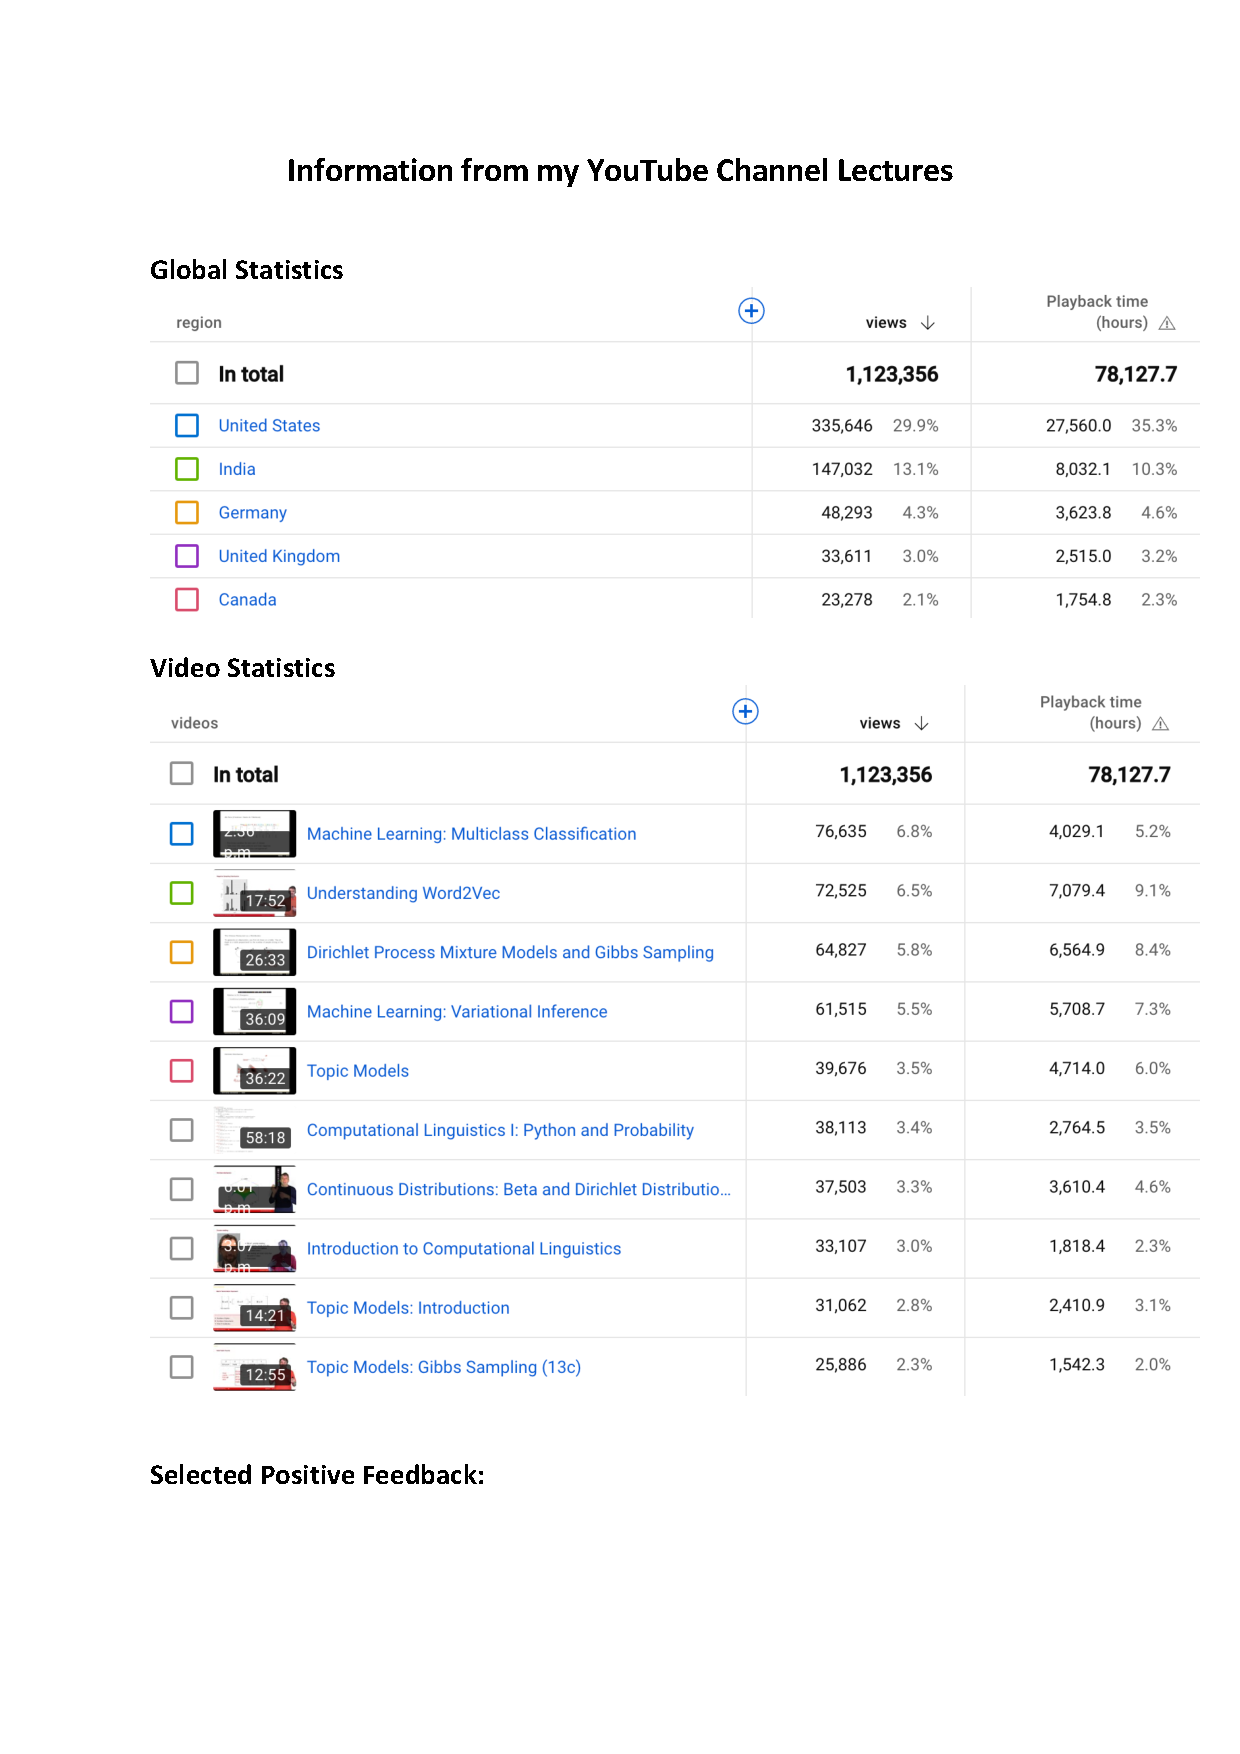
\includepdf[pages=1,pagecommand={\section{Statistics and Comments from YouTube}}]{resume_src/youtube}
\includepdf[pages=2-]{resume_src/youtube}

\clearpage

\bibliographystyle{resume_src/splncs03}

\bibliography{resume_src/journal-full,resume_src/jbg}
\noindent\rule{4cm}{0.4pt}

\end{document}

